
% \documentclass[blackref,approvalform,dvipsnames]{drexel-thesis}
\documentclass[draft,dvipsnames]{drexel-thesis}


\author{Jae Hoon Kim}
\title{This is the Title}
\DUTmonth{June}
\DUTyear{2017}
\degree{Master in Computer Science}
\advisor{Santiago~Onta\~{n}\'{o}n, Ph.D.}
\copyrighttext{\copyrighttextCCBYSA}

\usepackage[numbers,sort&compress]{natbib} % fancy citation extensions
\bibliographystyle{unsrtnat}


% \usepackage{fancyvrb} % nicer verbatim handling
% \DefineShortVerb{\|}  % \verb+TEXT+  ->  |TEXT|

\usepackage{xcolor}
\usepackage{colortbl,booktabs}
\usepackage{xspace}
\usepackage{multirow}
\usepackage{wrapfig} % text around figures
\usepackage{amssymb} % \mathbbstarcra
\usepackage[final]{listings} % algorithms formated in code
\usepackage{enumitem} % compact imte lists
\usepackage{subcaption} % for subfigure (figures side-by-side)
\usepackage{mathtools}
\usepackage{soul}
\usepackage[detect-all]{siunitx} % Aligning numbers by decimal points in table columns

\usepackage{algorithm, soul}
\usepackage[noend]{algpseudocode}
\algnewcommand{\Break}{\textbf{break}}

\newcommand{\todo}[1]{{\color{red}{\tt #1}}}
% \newcommand{\toredo}[1]{{\leavevmode\color{Plum}#1}}
\newcommand{\toredo}[1]{#1}
\newcommand{\modified}[1]{{\leavevmode\color{blue}#1}}
% \newcommand{\modified}[1]{#1}
\newcommand{\highest}[1]{\textcolor{Maroon}{\textbf{#1}}}
\newcommand{\StarCraft}{\mbox{\textsc{StarCraft}}\xspace}
\newcommand{\BroodWar}{\textsc{StarCraft: Brood War}\xspace}
\newcommand{\WarCraft}{\mbox{\textsc{WarCraft}}\xspace}
\newcommand{\WarCraftII}{\mbox{\textsc{WarCraft II}}\xspace}
\newcommand{\WarCraftIII}{\mbox{\textsc{WarCraft III}}\xspace}
\newcommand{\Wargus}{\mbox{\textsc{Wargus}}\xspace}
\newcommand{\Spring}{\mbox{\textsc{Spring}}\xspace}
\newcommand{\BWTA}{\textsc{BWTA}\xspace}
\newcommand{\BWTAb}{\textsc{BWTA2}\xspace}
\newcommand{\BWAPI}{\textsc{BWAPI}\xspace}
\newcommand{\SparCraft}{\textsc{SparCraft}\xspace}
\newcommand{\Lanchester}{\mbox{\emph{TS-Lanchester}$^2$}\xspace}
\newcommand{\cop}{\textsc{COP}\xspace}
\newcommand{\Ghost}{\textsc{GHOST}\xspace}
\newcommand{\Nova}{\textsc{Nova}\xspace}




\begin{document}
\begin{preamble}

% \begin{dedications}
% We're in \iffinal{final}{draft} mode!
% \end{dedications}

% \begin{acknowledgments}
% bla bla bla
% \end{acknowledgments}

\tableofcontents
\listoftables
\listoffigures

% \iffinal{}{\newpage}

\begin{abstract}
{\color{blue}[To do: Write an abstract here]}
\end{abstract}
\end{preamble}

\begin{thesis}



% ####################################################################################################################################
\chapter{Introduction}\label{chap:intro}
% ####################################################################################################################################

Introduction Section
\begin{enumerate}
\item Problem Statement
\end{enumerate}



% ====================================================================================================================================
% ====================================================================================================================================
\chapter{Background}\label{sec:bg}
% ====================================================================================================================================
% ====================================================================================================================================
This chapter presents the necessary background to understand the experiments presented later in the paper. This chapter is dived to three sections. First section \ref{sec:DL} covers basic deep learning including recurrent neural network and auto-encoder. Second section \ref{sec:DLL} compares deep learning libraries: DL4J, Theano, and Tensorflow. The last section \ref{sec:MLDD} introduces current trend of machine learning with driving data.

\section{Deep Learning}\label{sec:DL}
This section covers basic concept of deep learning. First subsection \ref{subsec:basicDL} introduces to deep learning, and next section \ref{subsec:RNN} deals with recurrent neural network and long short term memory neural network. The last subsection \ref{subsec:AE} covers auto-encoder.

\subsection{Basic Concept}\label{subsec:basicDL}
This part Explain basic deep learning

\subsection{Recurrent Neural Network}\label{subsec:RNN}

\begin{enumerate}
\item Basic concept of recurrent neural network

	A recurrent neural network (RNN) is a neural network that is specialized for processing a sequence of input values \cite{Goodfellow-et-al-2016}. The figure \ref{fig:RNN} illustrates abstract structure of RNN. RNN has two input. One input is from data such as normal neural network input but another input is from previous output and the property gives benefit for sequential input data. This is because past output affects to current output. With sequential data, previous data can affect to current data and RNN considers previous output for current output. It means that even input from data are equal if previous output are different, current output are also different.
	
\begin{figure}[t!]
    \centering
    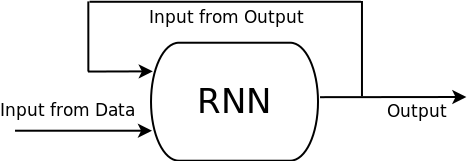
\includegraphics[width=0.65\textwidth]{pictures/figures/RNN.png}
    \caption{RNN}
    \label{fig:RNN}
\end{figure}
	
	For example, human language sentences have series of words and meaning of words is different in different context. RNN can be used for that. Another example is driving data which is used later on the paper.  Driving data are multi-dimension data with time domain. RNN can be used for the data because it is sequential data with time domain.
	
	To describe RNN in math equation, let $x^{t}$ be input data on time $t$, $h^{t}$ be result from hidden layer on time $t$, and $o^{t}$ be output on time $t$. The tensor $U$ is a set of neurons for input data, The tensor $V$ is a set of neurons for data from hidden layer and the tensor $W$ is a set of neurons for previous output. The figure \ref{fig:unfold_RNN} illustrates unfolded RNN with defined symbols. The value for hidden layer can be calculated by $h^{t} = Ux^{t} + Wo^{t-1}$ then the output can be calculated by $o^{t} = Vh^{t}$. Therefore, RNN can be written in $o^{t} = V(Ux^{t} + Wo^{t-1})$
	
\begin{figure}[t!]
    \centering
    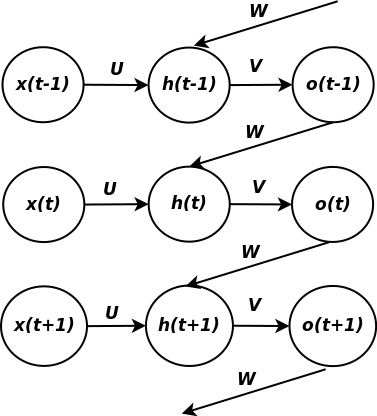
\includegraphics[width=0.5\textwidth]{pictures/figures/unfold_RNN.png}
    \caption{Unfold RNN}
    \label{fig:unfold_RNN}
\end{figure}


\item Long Short Term Memory (LSTM) networks:

	Basic RNN has problem of long term dependency. It means that RNN is not able to memorize long term knowledge. To solve the problem, LSTM is introduced by Hochreiter and Schmidhuber \cite{hochreiter1997long}. LSTM has cell state and it solves long term memory problem in RNN because cell state can store long term memory {\color{red} [santi: explain what is ``cell state'']}.
	
	Bengio mentioned on his paper \cite{bengio2009learning} that each layers in deep neural network should have {\color{red} a} purpose. LSTM can be divided to four layers: forget gate, input gate, input moduleation gate, and output gate. Each layers have different purpose {\color{red} [santi: this paragraph does not flow very well], even if Bengio mentioned it, why is it important? you need to explain WHY is it that each layer should have a purpose. Otherwise, we just have to blindly believe in Bengio :)}.
	
	{\color{red} [santi: this paragraph does not read very well, in blue below, I have an alternative version that flows better (just as an example)]}
	 Colah's blog \footnote{\url{http://colah.github.io/posts/2015-08-Understanding-LSTMs}} develops an intuition for concept of LSTM and explains purpose of each layer{\color{red} \st{s}}. The paper \cite{zaremba2014recurrent} describes LSTM in mathematical term{\color{red}s}. In this paper, I'm going to summarize both the Colah's blog and the paper \cite{zaremba2014recurrent}
	 
	{\color{blue} Let us first provide an intuitive description of how LSTMs work (following Christopher Olah's blog \footnote{\url{http://colah.github.io/posts/2015-08-Understanding-LSTMs}}), before providing a more in-depth formalization}:
	
	\begin{enumerate}
	\item An intuitive {\color{red} \st{concept} explanation} of LSTM{\color{red}s}:
	
		Colah's {\color{red} [santi: ``Colah'' $\to$ ``Christopher Olah'']} blog explains concept of LSTM and summarizes four layers in LSTM with each purpose. {\color{red} [santi: in LaTeX, the way to separate paragraphs is to leave a blank line between them, not using the double backslash (which should not be used often).]}
		
		The first layer is forget gate. The forget gate filters what data to forget or throw away. It consists of sigmod {\color{red} [santi: instead of saying ``It consists of sigmod'', you should say something like ``The units in this layer use a sigmoid activation function'' (same comment for all the other layers below)]} layer with previous output and current input data {\color{red} [santi: a reader not familiar with LSTMs will not know what is ``previous output'' or ``current input'', so you need a figure that explains it]}. The result of the forget gate is multiplied by previous cell state to build current cell state.
		
		The second layer is input gate and also consists of sigmod layer with previous output and current input data. The result of the input gate is multiplied by the result of input modulation gate then it affects to cell state {\color{red} [santi: all of these terms should appear in a figure, otherwise, a reader not familiar with it will not understand what you are saying. But also, even if you have a figure, you need to explain what each term is, e.g., explain what is ``input modulation'', what is ``cell state'', etc.]}. The meaning of input gate is to decide{\color{red} \st{s}} what data to remember.
		
		The third layer is input modulation gate. It consists of tanh with previous output and current input. It is multiplied by the result of second layer and affects to current cell state.
		
		The last layer is output gate. The layer decides what data should be passed to current output from previous output and current input. the output gate also consists of sigmoid with two inputs: last output and current input. The result of the layer is multiplied by current cell state passed tanh.
	
	\item Modeling LSTM in mathematical term{\color{red}s}:
		LSTM is described in mathematical term in the paper \cite{zaremba2014recurrent}. I'm going to summarize it on this paper.\\
	Let\\
	$T_{n,m}: \mathbb{R}^n \rightarrow \mathbb{R}^m$ be an affine transform\\
	$x_t$ be size $n$ vector for current input\\
	$h_{t-1}$ be size $n$ vector for last output \\
	$h_{t}$ be size $n$ vector for current output \\
	$c_{t-1}$ be size $n$ vector for last cell state \\
	$c_{t}$ be size $n$ vector for current cell state \\

\[
\begin{bmatrix}
    input\_gate \\
    forget\_gate \\
    output\_gate \\
    input\_modulation\_gate
\end{bmatrix}
=
\begin{bmatrix}
    i \\
    f \\
    o \\
    g
\end{bmatrix}
=
\begin{bmatrix}
    sigm & 0 & 0 & 0\\
    0 & sigm & 0 & 0\\
    0 & 0 & sigm & 0\\
    0 & 0 & 0 & tanh
\end{bmatrix}
T_{2n,4n}
\begin{bmatrix}
    h_{t-1} \\
    x_{t}
\end{bmatrix}
\]
\[
=
\begin{bmatrix}
    sigm & 0 & 0 & 0\\
    0 & sigm & 0 & 0\\
    0 & 0 & sigm & 0\\
    0 & 0 & 0 & tanh
\end{bmatrix}
\begin{bmatrix}
    {T^{hi}}_{n,n} & {T^{xi}}_{n,n} \\
    {T^{hf}}_{n,n} & {T^{xf}}_{n,n} \\
    {T^{ho}}_{n,n} & {T^{xo}}_{n,n} \\
    {T^{hg}}_{n,n} & {T^{xg}}_{n,n}
\end{bmatrix}
\begin{bmatrix}
    h_{t-1} \\
    x_{x}
\end{bmatrix}
\]
\[
=
\begin{bmatrix}
    sigm & 0 & 0 & 0\\
    0 & sigm & 0 & 0\\
    0 & 0 & sigm & 0\\
    0 & 0 & 0 & tanh
\end{bmatrix}
\begin{bmatrix}
    {T^{hi}}_{n,n}h_{t-1} + {T^{xi}}_{n,n}x_{x} \\
    {T^{hf}}_{n,n}h_{t-1} + {T^{xf}}_{n,n}x_{x} \\
    {T^{ho}}_{n,n}h_{t-1} + {T^{xo}}_{n,n}x_{x} \\
    {T^{hg}}_{n,n}h_{t-1} + {T^{xg}}_{n,n}x_{x}
\end{bmatrix}
\]
Therefore,\\
\[
\begin{bmatrix}
    i \\
    f \\
    o \\
    g
\end{bmatrix}
=
\begin{bmatrix}
    sigm({T^{hi}}_{n,n}h_{t-1} + {T^{xi}}_{n,n}x_{x}) \\
    sigm({T^{hf}}_{n,n}h_{t-1} + {T^{xf}}_{n,n}x_{x}) \\
    sigm({T^{ho}}_{n,n}h_{t-1} + {T^{xo}}_{n,n}x_{x}) \\
    tanh({T^{hg}}_{n,n}h_{t-1} + {T^{xg}}_{n,n}x_{x})
\end{bmatrix}
\]

$\{i, f, o, g\}$ is a set of output from each layers.
The current cell state $c_t = f \cdot c_{t-1} + i \cdot g$
the current output $h_t = o \cdot tanh(c_t)$

	\end{enumerate}
\end{enumerate}

\subsection{Auto-encoder}\label{subsec:AE}
In this section, I summarize 'Reducing the dimensionality of data with neural networks' by Hinton \cite{hinton2006reducing}. The paper introduces to the method to reduce high dimensional data by neural networks named auto-encoder. The result of the paper shows that reducing dimension by auto-encoder gives better performance than PCA. \\
\begin{enumerate}
\item Intuition concepts of auto-encoder\\
When auto-encoder is traind, it has two layers: encode and decode. The encode layer receives input and passes output in lower dimension data to decode layer. The decode layer recovers dimension to input data dimention from output of encode layer. The error of auto-encoder is measured by difference between input data and output from decode layer. In other words, encoder layer compresses input data and decoder layer decompresses data from encoder layer that should be similar as original input data. That methods guarantees that the data from encoder layer keeps almost all properties of input data in lower dimension. That is the reason why output data from decode layer is similar as original input data. In math, relationship between encoder and decoder layer is similar as inverse matrix of each other.

\item Multilayer Auto-encoder\\

\end{enumerate}

\section{Deep Learning Library}\label{sec:DLL}
\subsection{DL4J}
DL4J \footnote{\url{https://deeplearning4j.org/}} is open source, distributed deep-learning library for Java and Scala. It also integrates with Hadoop and Spark. 

\subsubsection{Theano}
Theano \footnote{\url{http://deeplearning.net/software/theano/}} is a Python library for machine learning research. It integrates with Numpy and uses GPU power. The library is written in C code and optimizes user functions.

\subsubsection{Tensorflow}
Tensorflow \footnote{\url{https://www.tensorflow.org/}} is an open source software library for numerical computation using data flow graphs. The biggest difference from other libraries is that Tensorflow treats all operator as node. Another strong point is that Tesorflow allows developer to deploy computation to one or more CPUs or GPUs. 


\section{Machine Learning with Driving Data}\label{sec:MLDD}

% ####################################################################################################################################
\chapter{Data Set}
% ####################################################################################################################################


The drive simulation data is from \textit{Children's Hospital of Philadelphia} (CHOP). The simulator for the data can record 100 features with 60 samples per second from driver. The simulator has four different tracks. On the paper, the data has 16 set: 8 from expert and 8 from inexpert. Each expert and inexpert data set consist of two set of four different tracks.

% ####################################################################################################################################
\chapter{Technical Approach}
% ####################################################################################################################################

\section{Cross Validation}
There are only 16 data set. It is not enough to train neural network for general case. Whether the neural network works well on the problem or not, I used cross validation. I split 16 data set to 4 groups. Each groups have 2 expert and 2 inexpert data. The neural network is trained four times with different train (3 groups) and test (1 group) set. 

\section{LSTM}
The LSTM neural network is used to classify data because the data has time domain and LSTM neural network can handle serial data. On the paper, LSTM neural network is built with 16, 32, 64, 128, and 256 hidden neurons. The output from LSTM is sent to output layer which has two neurons. By using softmax, output from two neurons is classified. If it has [0, 1], it is classified to expert. Otherwise, it is classified to inexpert.

\begin{figure}[H]
    \centering
    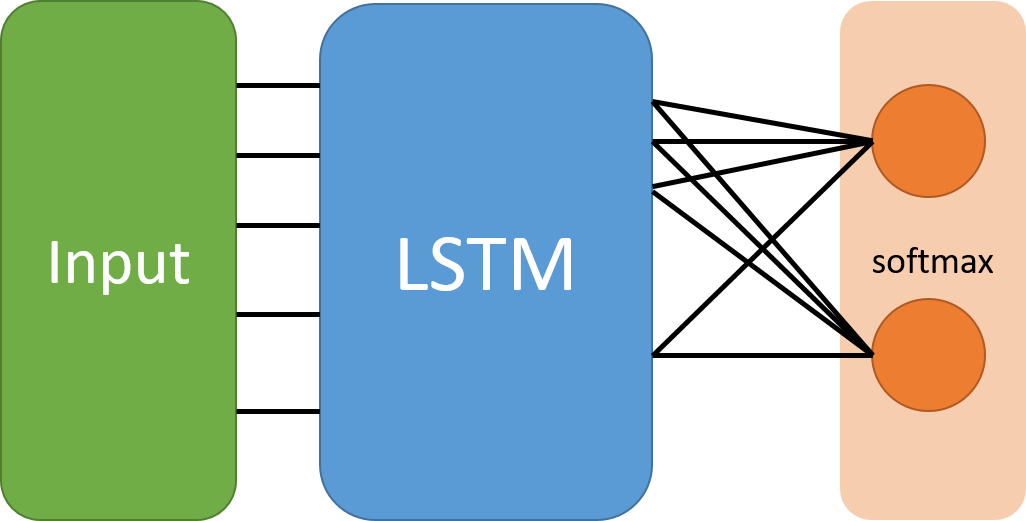
\includegraphics[width=0.5\textwidth]{pictures/applied_lstm.png}
    \caption{LSTM without Auto-Encoder}
    \label{fig:Applied LSTM}
\end{figure}

\section{Dimensionality Reduction}
The data has 100 features so dimensionality reduction is necessary. First way is selecting meaningful features and 23 features are selected. Another way to reduce dimension is auto-encoder. Before giving data to LSTM neural network, data is sent to auto-encoder layer and less dimension data from auto-encoder is sent to LSTM. 

\begin{figure}[H]
    \centering
    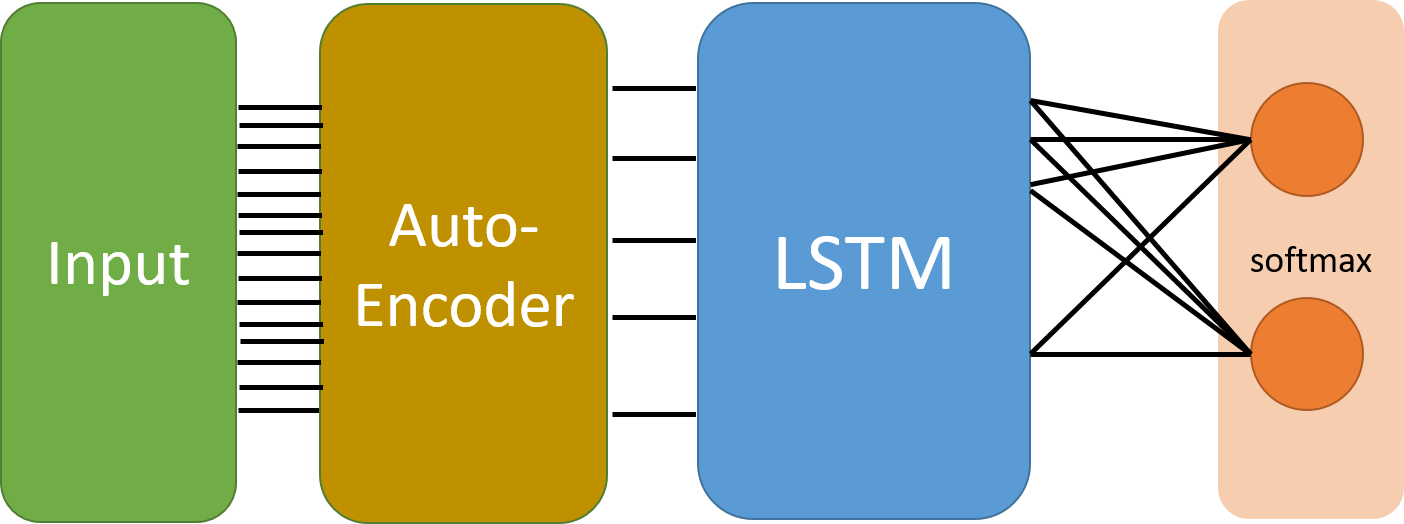
\includegraphics[width=0.5\textwidth]{pictures/applied_lstm_autoencoder.png}
    \caption{LSTM with Auto-Encoder}
    \label{fig:Applied LSTM With Auto-Encoder}
\end{figure}

%\subsection{Raw vs. Filtered data}

\section{Sampling}
The simulator records 60 samples per second. It is too often recorded. I reduce data by two way. First way is sampling one per ten and sampling one per twenty. The sampled data might not represent ten or twenty data, so average data from every ten or twenty data is used. The second way can reduce noise because there is case in first way that sampled data has more noise than other data.


% ####################################################################################################################################
\chapter{Experiment Result}
% ####################################################################################################################################


\begin{figure}[H]
    \centering
    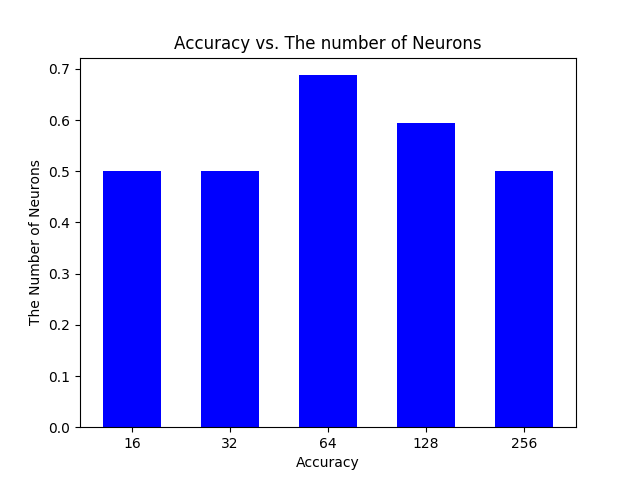
\includegraphics[width=0.75\textwidth]{pictures/accuracy.png}
    \caption{Accuracy}
    \label{fig:Accuracy}
\end{figure}


\begin{table}[H]
\centering
\begin{tabular}{|l|l|l|l|l|l|l|}
\hline
                       &      & \multicolumn{5}{l|}{The number of neurans} \\ \hline
Test                   & n    & 16    & 32    & 64      & 128      & 256   \\ \hline
\multirow{4}{*}{1}     & 1    & 0.5   & 0.25  & 1.0     & 0.5      & 0.5   \\ \cline{2-7} 
                       & 2    & 0.75  & 0.75  & 0.5     & 0.5      & 0.5   \\ \cline{2-7} 
                       & 3    & 1.0   & 0.5   & 0.5     & 0.75     & 0.5   \\ \cline{2-7} 
                       & 4    & 0.5   & 0.5   & 0.75    & 0.5      & 0.5   \\ \hline
\multirow{4}{*}{2}     & 1    & 0.5   & 0.75  & 0.75    & 0.75     & 0.75  \\ \cline{2-7} 
                       & 2    & 0.25  & 0.25  & 0.75    & 0.5      & 0.25  \\ \cline{2-7} 
                       & 3    & 0.5   & 0.5   & 0.25    & 0.75     & 0.25  \\ \cline{2-7} 
                       & 4    & 0.25  & 0.25  & 0.5     & 0.25     & 0.75  \\ \hline
\multirow{4}{*}{3}     & 1    & 0.75  & 0.25  & 1.0     & 0.75     & 0.25  \\ \cline{2-7} 
                       & 2    & 0.25  & 0.5   & 0.75    & 0.5      & 1.0   \\ \cline{2-7} 
                       & 3    & 0.5   & 0.75  & 0.75    & 0.5      & 0.5   \\ \cline{2-7} 
                       & 4    & 0.5   & 0.25  & 0.75    & 0.75     & 0.5   \\ \hline
\multirow{4}{*}{4}     & 1    & 0.75  & 0.5   & 0.5     & 0.5      & 0.5   \\ \cline{2-7} 
                       & 2    & 0.25  & 0.5   & 0.5     & 1.0      & 0.25  \\ \cline{2-7} 
                       & 3    & 0.0   & 0.75  & 1.0     & 0.75     & 0.25  \\ \cline{2-7} 
                       & 4    & 0.75  & 0.75  & 0.75    & 0.25     & 0.75  \\ \hline
\multicolumn{2}{|l|}{Average} & 0.5   & 0.5   & 0.6875  & 0.59375  & 0.5   \\ \hline
\end{tabular}
\caption{Raw 1/10 Result Summary}
\label{Raw 1/10 Result Summary}
\end{table}


% ####################################################################################################################################
\chapter{Conclusion and Future work}
% ####################################################################################################################################
Conclusion and Future work\\



\end{thesis}

\bibliography{references.bib}

\end{document}
\endinput

